
\section{État de l'art}

\subsection{\textit{A Review of Digital Terrain Modeling}\cite{DTMpaper}}
Ce papier de recherche fait un tour d’horizon des méthodes de génération de terrain par ordinateur. Le papier étant fourni nous nous attarderons uniquement sur les parties qui nous semblent les plus pertinentes.

\paragraph{Représentation du terrain}
La modélisation numérique d’un terrain repose sur une fonction d’élévation $h : \mathbb{R}^2 \rightarrow \mathbb{R}$ de classe au moins continue ($C^0$), qui associe une altitude à chaque point du plan. Cette définition suppose l’absence de surplombs, d’arcs ou de cavernes. Le terrain $T$ est défini sur un domaine $\Omega \subset \mathbb{R}^2$, souvent un rectangle $R(a, b)$ dont $a$ et $b$ sont des coins opposés. La pente en un point $p$ est donnée par la norme du gradient $\|\nabla h(p)\|$, tandis que la normale au terrain s’exprime par la projection $( -\nabla h(p), 1 )$ dans $\mathbb{R}^3$, puis normalisée.

L’élévation peut être représentée par une fonction explicite (analytique ou procédurale). Bien que cette approche soit compacte en mémoire et offre une précision théorique infinie, elle peut être coûteuse en calcul. En pratique, la représentation la plus courante est la grille régulière de valeurs d'altitude, appelée \textit{champ de hauteurs} (ou \textit{Digital Elevation Model}, DEM). Elle consiste en une grille 2D régulière sur laquelle les altitudes $z_{ij}$ sont échantillonnées aux points $p_{ij}$ selon une subdivision en $n$ intervalles. Cette méthode nécessite de reconstruire la surface terrain par interpolation (bilinéaire ou bicubique). L’interpolation bilinéaire assure une continuité $C^1$ à l’intérieur des cellules, mais seulement $C^0$ à leurs bords. Les interpolations d'ordre supérieur (par exemple bicubique) sont plus précises mais plus coûteuses en calcul.

\begin{figure}[!h]
    \centering
    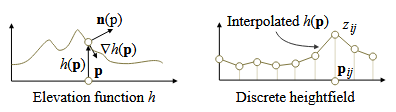
\includegraphics[width=0.6\linewidth]{images/DTM_elevation.png}
    \caption{Difference entre représentation explicite et champ de hauteur}
    \label{fig:enter-label}
\end{figure}

Bien que les champs de hauteurs soient plus gourmands en mémoire ($O(n^2)$), ils permettent de représenter divers reliefs, contrairement aux fonctions explicites. Des techniques comme la quantification (souvent en 8 ou 16 bits) sont utilisées pour réduire les besoins mémoire. Cependant, une précision de 8 bits est insuffisante pour des applications telles que la génération procédurale ou la simulation, car elle provoque des artefacts visuels. Les champs de hauteurs sont largement utilisés dans les outils de création de terrain, les simulations d’érosion, les jeux vidéo et l’industrie cinématographique (souvent combinés à des structures 3D plus complexes).

\paragraph{Génération procédurale de terrains}

Dans cette étude, on qualifie de \textit{procédurale} toute méthode de génération de terrain qui ne repose ni sur une simulation physique réelle (comme l’érosion hydraulique), ni sur l’utilisation de données issues du monde réel. Ces approches cherchent plutôt à reproduire directement les effets observés dans la nature, en s’appuyant sur des propriétés générales des terrains comme leur caractère fractal. Elles s’inspirent des formes naturelles, mais sans utiliser de données réelles comme exemples.

Les méthodes procédurales se divisent en deux grandes catégories. D’une part, la génération de terrains à grande échelle vise à synthétiser un relief sur l’ensemble du plan $\mathbb{R}^2$ ou un domaine étendu $\Omega \subset \mathbb{R}^2$. Ces méthodes exploitent les propriétés d’auto-similarité des reliefs à différentes échelles, mais offrent généralement peu de contrôle sur la forme finale. D’autre part, les méthodes de génération de formes de terrain spécifiques (par exemple collines, rivières ou canyons) travaillent à plus petite échelle et permettent un contrôle plus direct ou indirect sur la géométrie générée grâce à des paramètres ajustables.

\newpage

\paragraph{Génération à grande échelle par subdivision}

Les terrains naturels tels que les chaînes de montagnes érodées ou les littoraux présentent souvent des structures similaires aux propriétés fractales. De nombreux algorithmes de génération à grande échelle exploitent ces caractéristiques, produisant des détails qui se répètent à toutes les échelles.

Parmi ces algorithmes, les \textit{schémas de subdivision} raffinent itérativement une grille initiale pour ajouter des détails de plus en plus fins. L’un des plus connus est l’algorithme de déplacement de points médians (\textit{midpoint displacement}), qui introduit de nouveaux points en moyenne des voisins existants, puis applique un déplacement aléatoire dont l’amplitude décroît à chaque niveau d’itération, en fonction de la dimension fractale souhaitée.

Pour limiter les artefacts directionnels visibles (par exemple les pics aux premiers niveaux de subdivision), plusieurs variantes ont été proposées. Le schéma \textit{diamond-square} presenté dans la figure 7, bien que populaire, présente des extrema locaux visibles. Le schéma \textit{square-square} améliore cet aspect en équilibrant mieux les subdivisions. D’autres schémas utilisent des combinaisons de polygones (triangles, carrés...) pour conserver la cohérence géométrique et topologique lors du raffinement.

\begin{figure}[!h]
    \centering
    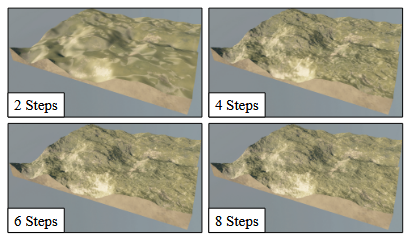
\includegraphics[width=0.6\linewidth]{images/DTM_diamond.png}
    \caption{Exemple algorithme diamond square}
    \label{fig:enter-label}
\end{figure}


\paragraph{Génération par fonctions de bruit}

Les fonctions de bruit sont largement utilisées dans la génération procédurale de terrains. Elles permettent de modéliser des reliefs variés en combinant plusieurs bruits à différentes échelles et amplitudes. L’un des modèles les plus courants est le mouvement brownien fractionnaire (fBm)\cite{brow}, obtenu en sommant plusieurs octaves d’une fonction de bruit lisse avec des fréquences et amplitudes variables. Ces paramètres, appelés \textit{lacunarity} et \textit{persistence}, influencent respectivement la variation de fréquence et d’amplitude d’une octave à l’autre, et donc l’aspect global du terrain : plus rugueux ou plus doux.

Pour simuler des crêtes ou des arêtes plus marquées, des variantes comme le \textit{ridge noise} (ou bruit de crête) inversent la forme du bruit pour créer des sommets nets, adaptés aux chaînes de montagnes jeunes.

\begin{figure}[!h]
    \centering
    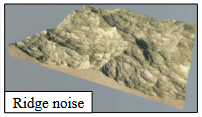
\includegraphics[width=0.35\linewidth]{images/ridge_noise.png}
    \caption{Exemple bruit de crête}
    \label{fig:enter-label}
\end{figure}

D’autres extensions, comme le \textit{bruit multifractal}, modifient dynamiquement l’amplitude des octaves selon l'altitude locale, afin de mieux reproduire les différences entre plaines douces et montagnes accidentées.

\begin{figure}[!h]
    \centering
    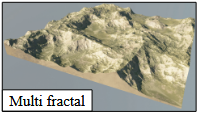
\includegraphics[width=0.35\linewidth]{images/multi_fractal_noise.png}
    \caption{Exemple bruit multifractal}
    \label{fig:enter-label}
\end{figure}

Enfin, pour éviter les artefacts de grille souvent visibles dans les sommes simples de bruits, on applique des transformations appelées \textit{warping} (enroulé) au domaine d’entrée de la fonction. Cela permet de déformer le terrain de manière plus organique.

\begin{figure}[!h]
    \centering
    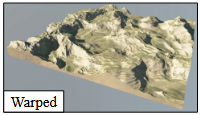
\includegraphics[width=0.35\linewidth]{images/wraped.png}
    \caption{Exemple bruit multifractal avec enroulage}
    \label{fig:enter-label}
\end{figure}

Bien que ces techniques puissent imiter certains effets d’érosion, elles restent des approximations, et des simulations physiques plus complexes sont nécessaires pour des résultats réalistes. La figure 8 montre des exemples d'application de ces méthodes pour la génération de terrain.



 \paragraph{Limites des approches fractales pour la génération de terrains}

Les approches basées sur la subdivision ou les fonctions de bruit sont couramment utilisées pour générer des terrains synthétiques à grande échelle, en raison de leurs fortes propriétés fractales. Toutefois, ces méthodes peinent à reproduire les structures de haut niveau que l’on observe dans les terrains réels, comme les ramifications caractéristiques des chaînes de montagnes. Les fonctions de bruit offrent une grande flexibilité, notamment grâce aux techniques de déformation (warping), de lissage ou de combinaison, mais leur contrôle reste complexe et nécessite à la fois une bonne maîtrise technique et un sens artistique développé. À l'inverse, les méthodes par subdivision, bien que plus simples à manipuler, sont moins présentes dans les outils industriels, principalement en raison de leur moindre compatibilité avec le calcul parallèle.

L’un des avantages majeurs des fonctions de bruit réside dans leur capacité à être évaluées indépendamment pour chaque point, ce qui les rend particulièrement efficaces sur GPU pour l’édition interactive. Néanmoins, cette indépendance constitue aussi une limite importante : ces fonctions ne tiennent pas compte des relations locales entre les points, et ne permettent donc pas de modéliser des phénomènes complexes tels que le transport de matière ou l’érosion. En outre, le caractère strictement fractal de ces méthodes ne correspond pas à la diversité morphologique réelle des paysages, ce qui restreint leur réalisme à certaines échelles ou à des formes spécifiques comme les côtes fractales. Ces limites ont conduit la recherche à se tourner vers des modèles plus spécialisés, capables de générer des formations géographiques précises tout en conservant les performances des approches procédurales.

\paragraph{Méthodes de génération basées sur les entités géographiques}

Les méthodes dites "feature-based" reposent sur la modélisation explicite de structures géographiques clés comme les crêtes, les vallées ou les lits de rivières. Deux grandes approches se distinguent : d'une part, les techniques basées sur des courbes de contrôle permettent à l’utilisateur de dessiner les grandes lignes du relief à partir de profils et de silhouettes, qui guident ensuite la déformation du terrain. Ce type de modélisation, souvent interactif, permet une grande expressivité et un contrôle précis sur la forme finale du terrain. D’autre part, les méthodes par "arbres de construction" combinent des primitives de terrain (comme collines, montagnes, rivières) hiérarchiquement à l’aide d’opérations de fusion ou de déformation. Ces approches permettent de construire des terrains complexes en associant des éléments topographiques à différentes échelles. En s’appuyant sur des structures géographiques réelles (réseaux hydrographiques, pentes, courbures), ces méthodes offrent un compromis intéressant entre contrôle utilisateur, réalisme géomorphologique et potentiel procédural.


\paragraph{Conclusion}
L'étude des méthodes présentés par cet article nous a permis de connaître les méthodes qui existent pour générer du terrain par ordinateur, leurs avantages et inconvénients. Nous avons explorés ces pistes pour creer notre carte.